%%%%%%%%%%%%%%%%%%%%%%%%%%%%%%%%%%%%%%%%%%%%%%%%%%%%%%%%%%%%%%%%%%%%%%%%%%%%%%%%%%%%%
% Reinforcement Learning
%
% Introduction to MDPs, finite MDPs, infinite MDPs
% Semi MDPs
% Partially Observable MDPs
%
%%%%%%%%%%%%%%%%%%%%%%%%%%%%%%%%%%%%%%%%%%%%%%%%%%%%%%%%%%%%%%%%%%%%%%%%%%%%%%%%%%%

\section{The Reinforcement Learning Problem}

In general terms, reinforcement learning in an industrial setting is simply an agent undergoing meaningful interactions with the process to learn an optimal operating policy.  For added intuition, Figure \ref{fig: simple_rl} shows the information flow of an agent in process control. First, the agent observes some states, $x_t \in \mathcal{X}$, from the environment (some states may be unobservable).  Given $x_t$, the agent performs some controls actions, $u_t \in \mathcal{U}$ and receives a scalar reward signal, $r_{t+1} \in \mathcal{R}$.  Finally, the process will transition to some new states, $x_{t+1}$, given probability $P(x_{t+1}, r_{t+1} | x, u)$.

\begin{figure}[H]
    \centering
    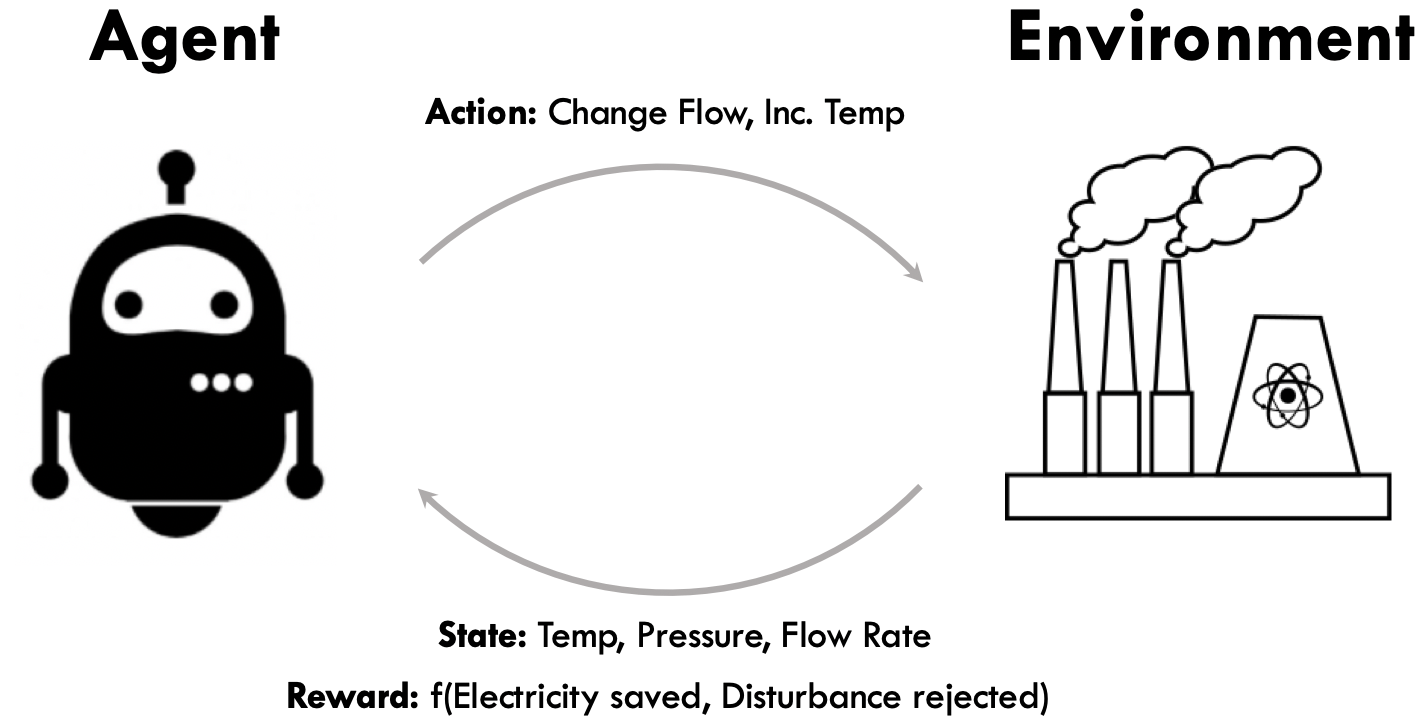
\includegraphics[scale=0.5]{images/ch1/RL.png}
    \caption{Basic setup of reinforcement learning where an agent interacts with the system.}
    \label{fig: simple_rl}
\end{figure}

The three main branches of reinforcement learning solutions are shown in Figure \ref{fig:RL_methods}. Starting from the left, dynamic programming (DP) methods can identify the exact value functions, but require a \textit{perfect system model} and is extremely computationally expensive, even for trivial tasks.  Comparatively, both Monte Carlo (MC) and temporal difference (TD) methods are approximate DP methods.  As such, they are less computationally demanding.  Additionally, MC and TD methods do not assume the presence of a system model and identifies the value functions through interactions with the environment. MC methods find the value functions through averaging the returns generated over many sampled trajectories of states, actions, and rewards.  One drawback is the significant variance in the sampled trajectories. Consequently, this may lead to poor reproducability in highly noisy systems. TD methods combine the best characteristics of DP and MC methods into one unifying approach. Like MC methods, TD learn from sampled data.  Like DP methods, TD performs update steps after each step. However, TD methods typically exhibit large bias (especially during initial learning episodes) due to estimating values through previously estimated values (known as bootstrapping). The general details of each method will be shown throughout this section.  For a comprehensive introduction to each algorithm, see \cite{sutton}.

\begin{figure}[H]
    \centering
    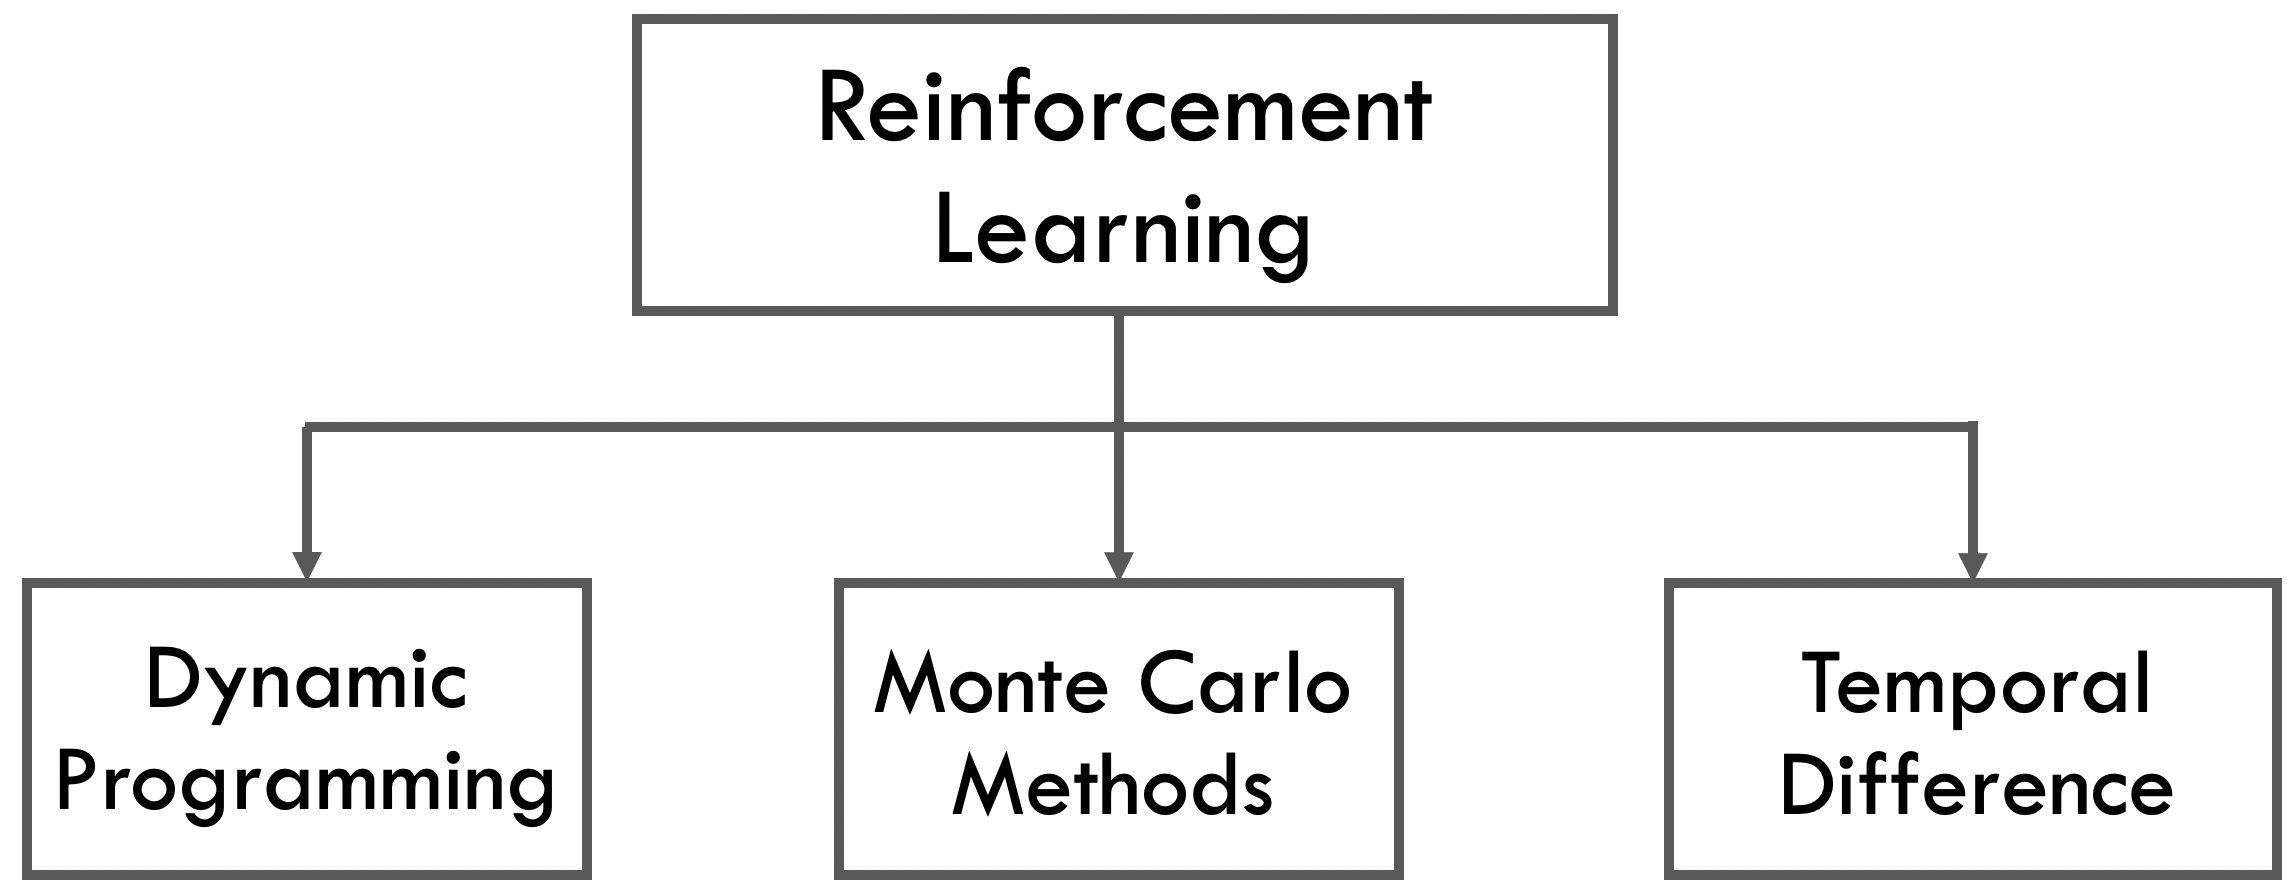
\includegraphics[width=0.6\textwidth]{images/ch1/RL_methods.jpeg}
    \caption{The sub-components of machine learning.}
    \label{fig:RL_methods}
\end{figure}   


\subsection{Dynamic Programming Methods}
Dynamic programming algorithms identify the exact value functions through an iterative procedure using the system dynamics function. In real life applications, DP algorithms are rarely used due to their unreasonable computational cost for even trivial problems. Nevertheless, the ideas of DP serve as the fundamentals for modern approaches. Policy iteration and value iteration are two common techniques in DP.  

As an overview, policy iteration searches for the optimal policy by iterating through infinitely many policies, $\pi \in \Pi$, storing only the policy corresponding to the highest cumulative returns.  The optimal policy is assumed to be found when $G_{\pi}$ can no longer be improved.  Policy iteration is comprised of two phases: policy evaluation and policy improvement. \textbf{Policy evaluation} computes the value functions and cumulative returns of the system under $\pi$ through an iterative approach. Value functions are initialized as 0, and are solved iteratively using:
\begin{equation}
    v_{k+1, \pi}(x) = \mathbb{E}_{\pi}[R_{t+1} + \gamma v_{k, \pi} (x_{k+1})]
\end{equation}
$$ v_0(x) = 0, \; \forall x \in \mathcal{X}$$
where $k$ denotes the $k^{th}$ update.  Here, $v_{k+1, \pi}(x)$ is the predicted value function for $x$ under policy $\pi$ after $k+1$ update steps.  As $k \rightarrow \infty$, $v_{k}(x) \rightarrow v_{\pi}(x)$ for all $x \in \mathcal{X}$ (i.e., the value functions converge to the true value functions under $\pi$). However, there often exists a $\pi'$ where $v_{\pi'}(x) \geq v_{\pi}$.  \textbf{Policy improvement} identifies such situations.  Once identified, current policy $\pi$ will violate the principle of optimality, hence deeming it ineligible for being the optimal policy. Then, the value functions of $\pi'$ will be identified in the next policy evaluation. This procedure will continue iteratively and infinitely until a policy where $v_{\pi^*}(x) \geq v_{\pi \neq \pi^*}(x)$ for all $x \in \mathcal{X}$ is found. After such a policy is identified, it is regarded as the optimal policy.

Figure \ref{fig:policy_iteration} shows a visualization of the policy iteration algorithm.  It can also be described using the following \cite{sutton}:
\begin{equation}
    \pi_0 \xrightarrow{\text{E}} 
    v_{\pi_0} \xrightarrow{\text{I}} 
    \pi_1 \xrightarrow{\text{E}}
    v_{\pi_1} \xrightarrow{\text{I}} 
    \pi_2 \xrightarrow{\text{E}} ... \xrightarrow{\text{I}} 
    \pi^* \xrightarrow{\text{E}}  v^*
\end{equation}
where $\xrightarrow{\text{E}}$ and $\xrightarrow{\text{I}}$ denotes the policy evaluation and policy improvement steps, respectively. From Figure \ref{fig:policy_iteration}, the agent starts with some arbitrary policy and performs policy evaluation. Initially, a large gap exists between $V_{\pi}$ and $\pi$.  As the iterative procedure proceeds, the gap is continuously reduced until $V_{\pi}, \pi \rightarrow V^*(x), \pi^*$. In industrial applications, the required iterative procedure for each policy evaluation is far too expensive for any non-trivial tasks.

\begin{figure}[H]
    \centering
    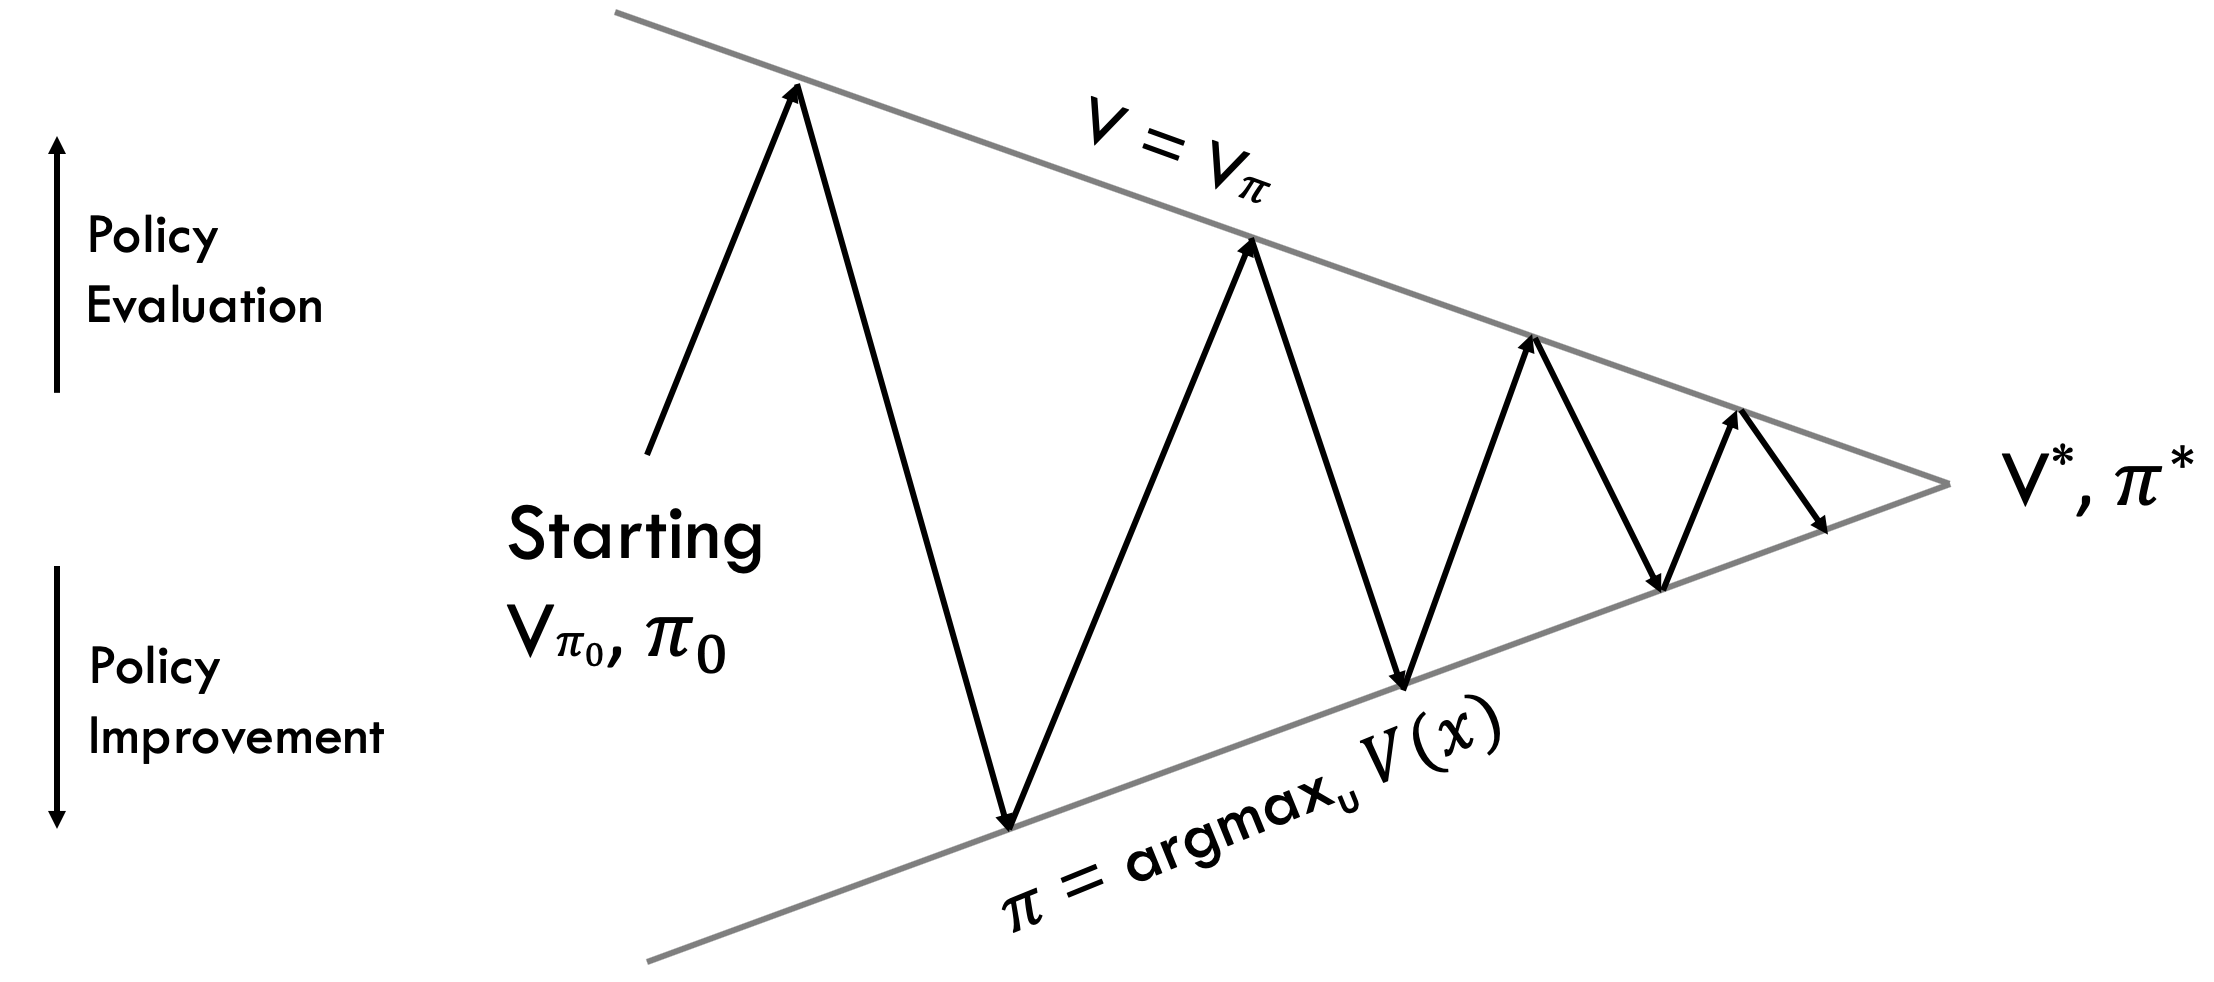
\includegraphics[width=0.68\textwidth]{images/ch1/policy_iteration.jpeg}
    \caption{A visualization of the policy iteration algorithm. Original image from \cite{silver_class}.}
    \label{fig:policy_iteration}
\end{figure}   

To improve upon these computational issues, value iteration was proposed.  Value iteration finds the optimal policy through identifying the optimal value functions instead. Intuitively, value iteration is a special case of policy iteration where the policy evaluation is terminated after one step.  From the value functions of each state, $\pi^*$ can be found by traversing through the states corresponding to the highest values. Note that the optimal policy can only be found using $V(x)$ if a dynamics equation of the system is provided. Without it, $Q(x, u)$ must be identified instead to behave optimally. The policy evaluation for the value iteration algorithm is given as:
\begin{equation}
    v_{k+1}(x) = \max_u \mathbb{E}[R_{t+1} + \gamma v_k(x_{t+1})]
\end{equation}
\begin{equation}
    q_{k+1}(x, u) = \mathbb{E}[R_{t+1} + \gamma \max_{u_{t+1}} q_k(x_{t+1}, u_{t+1})]
\end{equation}
Here, the $max$ operation ensures that each $v_k(x)$ is updated using only the maximizing action so the \textit{optimal} value function can be identified. After all $v^*(x)$ are identified, an agent can behave optimally starting in any state assuming the agent takes the maximizing action at each time. Note that both policy and value iteration are \textit{bootstrap} methods. Bootstrapping in RL increases data efficiency while capturing long-term trajectory information; however, the method also introduces unintended biased. 

In industry, both policy and value iteration have limited utility because their updates are far too computationally expensive. In high dimensional settings, even one iterative step may be intractable; therefore, even with value iteration's reduced computational complexity, it is still infeasible for most complex problems. Asynchronous dynamic programming methods further reduces computational complexity by only updating frequently visited states. However, agents are rendered hopeless in states that are rarely encountered. Although, such a methodology mimics human behaviour where encounters can be handled effectively and efficiently and more exotic situations may catch us by surprise. Nonetheless, such methods still require system models to be explicitly provided, a extremely rare case in industry.

\subsection{Monte Carlo Methods}
Monte Carlo methods no longer require explicit system models (a characteristic known as \textit{model-free}).  Instead, MC methods \textit{estimate} the average returns for different policies through sampling infinitely many sequences of states, actions, and rewards. As the samples increase, $v_k(x) \rightarrow v_{\pi}(x) \text{ for all } x \in \mathcal{X}$. Learning-wise, the average returns are updated at the end of each trajectory. Due to this, the finite tasks with explicit terminal states are typically solved using MC methods. For example, discrete manufacturing is an episodic task in process control. The system is reset after the assembly of each object (cars, toys, ...).  In episodic tasks, the value functions are updated naturally after each episode. However, most tasks in process control are continuous. Training a continuous agent using MC methods require additional modifications. One method is to pre-specify a length of time. After the time has elapsed, the agent will pause and update its value functions. 

Policy search in MC methods is similar to policy iteration. There exists three differences: 1) only visited states are updated; 2) updates use \textit{sampled} data instead of a model; 3) $q_{\pi}(x, u)$ is required and identified instead of $v_{\pi}(x)$. In MC methods, the action-value functions are identified because a model is not provided to the agent. Hence, the agent cannot behave optimally using only the value functions because the actions required to transition to the high value states are not known. Instead, action-values contain explicit information on the expected returns for each action in each state.  The iterative procedure of MC to compute the cumulative returns is given by: 
\begin{equation}
    \pi_0 \xrightarrow{\text{E}} 
    q_{\pi_0} \xrightarrow{\text{I}} 
    \pi_1 \xrightarrow{\text{E}}
    q_{\pi_1} \xrightarrow{\text{I}} 
    \pi_2 \xrightarrow{\text{E}} ... \xrightarrow{\text{I}} 
    \pi^* \xrightarrow{\text{E}}  q_{\pi_*}
\end{equation}
Intuitively, the agent is initiated in an unknown system and follows a certain policy, $\pi$, to traverse throughout the state space while collecting rewards after each decision. Eventually, the agent will reach a terminal state and conclude the episode. Upon termination, a sequence of returns $G_1, G_2, ..., G_{n - 1}$ can be generated using the received reward signals:
$$G_1 = R_{1} + \gamma R_{2} + \gamma^2 R_{3} + ... + \gamma^{n - 1}R_{n}$$
$$G_2 = R_{2} + \gamma R_{3} + \gamma^2 R_{4} + ... + \gamma^{n - 2}R_{n}$$
$$G_3 = R_{3} + \gamma R_{4} + \gamma^2 R_{5} + ... + \gamma^{n - 3}R_{n}$$
$$\vdots$$
$$G_{n - 1} = R_n$$
or:
\begin{equation}
    G_m = \sum\limits_{i=0}^n \gamma^{i} R_{m + i}
\end{equation}
where $G_m$ denotes the discounted cumulative return received on the $m^{th}$ step. Using $G_m$, the action-values can be computed for each step by:
\begin{equation}
    Q_{k+1}(x, u) = Q_{k}(x, u) + \frac{1}{k} \left[G - Q_k(x, u) \right]
    \label{eq:q_update_mc}
\end{equation}
where $Q_k(x, u)$ represents the $k^{th}$ action-value update and $G$ corresponds to the returns received after performing action $u$ in state $x$. Notice that as $k \rightarrow \infty$, $\frac{1}{k} \rightarrow 0$; therefore, this set-up is ineffective in non-stationary settings because the updates get infinitely small.  To extend Equation \ref{eq:q_update_mc} to non-stationary problems, $\frac{1}{k}$ is changed to a constant given by $\alpha$:
\begin{equation}
        Q_{k+1}(x, u) = Q_{k}(x, u) + \alpha \left[G - Q_k(x, u) \right]
        \label{eq:01mcupdate}
\end{equation}
where $\alpha \in (0, 1]$ is known as the learning rate (also called step size). The lower bound prevents $\alpha$ from approaching 0; therefore, allowing for continually adaptation in non-stationary problems. After each update of Equation \ref{eq:01mcupdate}, a new episode starts and the procedures are repeated.  As $k, \text{ \# of episodes } \rightarrow \infty, Q(x, u) \rightarrow q(x, u)$. Once $Q(x, u)$ converge, online action selection can be conducted by:
\begin{equation}
    \pi^*(x) = \argmax_{u} q(x, u)
    \label{eq:policy_extract}
\end{equation}
That is, $\pi^*$ is performing the greedy action in each state.  

\subsubsection{Exploration in MC}
Notice that bootstrapping is not used in MC methods.  In fact, all value functions are estimated independently. As such, MC methods do not suffer from bias issues; however, MC methods may suffer from large variances instead caused by the noise in each sampled trajectory \cite{sutton}. Moreover, exploration is mandatory in MC methods because the dynamics of the system are unknown to the agent. Through exploration, the agent can discover the dynamics of the system and the value functions for each state.  Typically, exploration in MC methods is conducted by initiating the agent in a random state at the beginning of each episode. After infinite episodes, all states will be visited infinitely many times.

MC methods allow the agent to learn solely from sampled data; however, the action-values are updated only after each episode. Such a procedure is unnatural in continuous systems (most systems in process control), disadvantageous long episode systems, and is not intuitive to human behaviour. For example, humans learn immediately after feedback, not in pre-set increments. Temporal difference methods combine the best features of DP and MC methods into one unifying algorithm.





\subsection{Temporal-Difference Methods}
Temporal difference (TD) methods are mathematically simple and cheap computationally compared to MC and DP methods. TD methods learn from experiences (like MC methods) and bootstraps (like DP methods). Furthermore, a dynamics model is not required in TD methods. Instead, the agent learns the dynamics from interactions. Moreover, TD methods update their value functions immediately after $x_{t+1}$ and $R_{t+1}$ are received. The TD update algorithm for value and action-value functions are given in Equations \ref{eq:td_value} and \ref{eq:td_action_value}, respectively \cite{td}:
\begin{equation}
    V(x_t) \leftarrow V(x_t) + \alpha \left[R_{t+1} + \gamma V(x_{t+1}) - V(x_t) \right]
    \label{eq:td_value}
\end{equation}
\begin{equation}
    Q(x_t, u_t) \leftarrow Q(x_t, u_t) + \alpha \left[R_{t+1} + \gamma Q(x_{t+1}, u_{t+1}) - Q(x_t, u_t) \right]
    \label{eq:td_action_value}
\end{equation}
where $\leftarrow$ is the update operator. At each update, the old value function is corrected as a function of the \textit{TD error} by a fixed amount determined by $\alpha$.  The TD errors are at each time $t$ is given as:
$$\delta_t = R_{t+1} + \gamma V(x_{t+1}) - V(x_t)$$
$$\delta_t = R_{t+1} + \gamma Q(x_{t+1}, u_{t+1}) - Q(x_t, u_t)$$
The first two terms, $R_{t+1} + \gamma V(x_{t+1})$, denote the predicted value function for $x$ in accordance with the last interaction.  $V(x_t)$ is the previously predicted value function for $x$. After infinitely many interactions with the system,  $V(x_t) \rightarrow v(x_t)$ (i.e., the estimated values converge to the true values). The action-values follow the same procedure. After convergence of the values and/or action-values, the optimal action selection is given in Equation \ref{eq:policy_extract}.

\subsubsection{Exploration in TD}
Like MC methods, TD methods are also \textit{model-free}; therefore, action-values are required for the agent to act optimally and exploration is mandatory. A simple and common exploration method used in TD methods is the $\epsilon$-greedy action selection. Here, the agent performs the greedy action with a $\epsilon \in [0, 1]$ probability of performing a random action. During training, $\epsilon$ is typically decayed throughout training.  At the beginning, $\epsilon$ starts at a high value because agent knows nothing. Eventually, $\epsilon$ decays to a low value when training is almost complete. 

Unfortunately, random exploration is sample inefficient and may require the agent to undergo thousands of interactions before learning anything meaningful. Learning can typically be significantly accelerated through a heuristics function $\mathcal{H}: \mathcal{X} \times \mathcal{U} \rightarrow \mathbb{R}$ \cite{harl}.  One such heuristics approach is the upper confidence bound (UCB) action selection algorithm \cite{ucb}. Here, exploration is promoted on states that have high potential to be optimal and is given by:
\begin{equation}
    U_t = \argmax_u [Q_t(x, u) + \mathcal{H}] 
    \label{ucb}
\end{equation}
The heuristics function here is given by:
\begin{equation}
    \mathcal{H} = c \sqrt{\frac{ln \; t}{N_t(x, u)}}
\end{equation}
where $c$ is the degree of exploration.  Large $c$ values promote greater degrees of exploration. Furthermore, $N_t$ is the number of times action $u$ was selected prior to time $t$. As $N_t(x, u) \rightarrow \infty$, the corresponding $Q(x, u)$ has been updated many times and becomes very accurate.  Hence, the heuristics function $\mathcal{H} \rightarrow 0$. 

\subsubsection{Popular TD algorithms}
The two most popular TD algorithms are \textbf{SARSA} and \textbf{$Q$-learning}.  \textbf{SARSA} is an \textit{on-policy} algorithm. In such algorithms, the \textit{behaviour policy} and \textit{target policy} are identical.  Target policy refers to the goal policy of the agent.  Typically, this is the optimal policy.  Conversely, the behaviour policy, $b(u|s)$, is the policy used by the agent for decision making. In cases where the target and behaviour policy are identical, the agent is \textit{on-policy}. One flaw with \textit{on-policy} agents (assuming the target policy is the optimal policy) is that during training, the agent may quickly converge to a local optimum and never explore (since any policies containing exploration is not the optimal policy).  Ultimately, this results in a sub-optimal solution.  Contrarily, \textit{off-policy} agents, like \textbf{$Q$-learning}, typically follow exploratory policies during training to conduct deep exploration.  Then in online applications, the policy is swapped to the optimal policy. Moreover, \textit{off-policy} agents are \textit{guaranteed} to find the optimal policy assuming each state-action pair is visited infinite times and $b(u^* | s) > 0$ (i.e., probability of picking the optimal action under the behaviour policy is not 0) \cite{td}.

Since SARSA is \textit{on-policy}, the action-value function are updated using Equation \ref{eq:td_action_value} using the quintuple $(x_t, u_t, R_{t+1}, x_{t+1}, u_{t+1})$. $Q$-learning updates use only four parameters $(x_t, u_t, R_{t+1}, x_{t+1})$ through Equation \ref{eq:q_learning}:
\begin{equation}
    Q(x_t, u_t) \leftarrow Q(x_t, u_t) + \alpha \left[R_{t+1} + \gamma \argmax_{u_{t+1}} Q(x_{t+1}, u_{t+1}) - Q(x_t, u_t) \right]
    \label{eq:q_learning}
\end{equation}
In $Q$-learning, $u_{t+1}$ is not required because the action taken might follow a different policy compared to the target policy since the algorithm is \textit{off-policy}. Instead, Equation \ref{eq:q_learning} uses the $max$ operation to ensure $Q$-values are still updated towards the optimal policy. Ultimately, TD methods unify DP and MC methods, allowing the agent to learn from experiences and perform inter-episode updates to exploit the most recent learnings.

A detailed numerical example is provided in Chapter 4 where a tabular $Q$-learning algorithm was applied onto an industrial VFD system to conduct set-point tracking control.


\section{Reward design for process control}
The agent's reward function design for process control applications is similar to MPC.  For a regulation or set-point tracking problems, the MSE reward function can be used:
\begin{equation}
    r(x, u) = -(x_i - x_{sp})^2
\end{equation}
However, the agent may find it difficult to distinguish between small off-sets using this reward function.  For example, when the tracking error is 10, the reward is -100.  However, if the off-set was only 0.25 or 0.1, the agent would find it difficult to distinguish between the small rewards because the magnitude is significantly different compared to an error of 10.  One way to enhance the distinction is to use a Huber loss given as \cite{huber}:
\begin{equation*}
    r(x, u) = \begin{cases}
    x_t - x_{sp} & \quad if \; |x_t - x_{sp}| > 1 \\
    (x_t - x_{sp})^2 & \quad otherwise
    \end{cases}
\end{equation*}
In this case, large errors are not squared to significantly reduce their magnitude.  In the tabular cases, this error works exceptionally well; however, not so much in deep RL.  Typically, the inputs to neural networks must be normalized for it to learn sufficiently \cite{NN}.  When normalizing the rewards, small errors will once again become indistinguishable.  In such a case, the following reward function can be used:
\begin{equation*}
    r(x, u) = \begin{cases}
    x_t - x_{sp} & \quad if \; |x_t - x_{sp}| > 1, \\
    (x_t - x_{sp})^2 & \quad if \; 1 > |x_t - x_{sp}| > \eta, \\
    +1 & \quad otherwise
    \end{cases}
\end{equation*}
where $\eta$ is the minimum acceptable tracking error. Here, as the agent achieves control within $\eta$, the reward is significantly increased, causing the agent to heavily favor that operating region.  Such an idea is similar to zone MPC, where the objective of the controller is to guide the trajectory within a zone \cite{zone_mpc}. Another flaw with deep RL is its variance in the output actions.  For example, if the temperature inside a house varies between $\ang{22.1}$ C or $\ang{22.2}$ C, a human would not go and change the air conditioning set-point because the two temperatures are relatively the same.  In deep RL's case, these are seen as two different states, and correspond to different actions.  One could design a filter to remove such small actions from being sent to the system; however, one natural way to mitigate this is to add another cost in the reward function:
\begin{equation}
    r(x, u) = -[(x_t - x_{sp})^2 + \nu \Delta u_t^2]
\end{equation}
where $\Delta u_t$ is the change in input in the last sampling time. The coefficient, $\nu$, is used to tune the effect of the action on the reward.  For example, if the system's input signals are typically small, a large $\nu$ would be used so the tracking error does not dominate the entire reward function.

If the optimal input is known, the reward function can be designed as:
\begin{equation}
    r(x, u) = -[(x_i - x_{sp})^2 + (u_i + u_{ss})^2]
\end{equation}
Although such scenarios would be rare in industry. 

Lastly, the reward is sometimes clipped to avoid large TD errors causing numerical issues during bootstrapping \cite{reward_clip}.  From Equation \ref{eq:q_learning}, it can be seen that if a large reward was obtained,



\section{Summary of the different solution approaches}
The main features of DP, MC and TD methods are summarized in Table \ref{tab:dc_mc_td}. Overall, DP requires a dynamics function of the system to compute the value functions while both MC and TD methods can learn directly from interactions with the system. Both DP and TD methods use bootstrapping to estimate value functions, that is, they estimate the current value function based on previously estimated values. Bootstrapping is data efficient, but introduces large bias to the estimated values, especially in the early episodes.  Conversely, MC methods estimate the value functions of each state independently through sampling many system trajectories.  However, this method, instead, introduces high variance. For extremely noisy systems, the reproducability of the results may be difficult. Comparing the computational cost, DP methods require much more compared to MC or TD since all value functions are simultaneously solved. In MC methods, only the value functions that were visited in the sampled trajectories are updated.  Additionally, updates are conducted at the end of each episode and not after each step. Similar to DP methods, TD methods update the value function immediately after an experience; however, only the value function corresponding to the last visited state is updated. In terms of exploration, DP methods do not explore the system model (both transition probabilities and expected reward) is explicitly provided. MC methods explore by being initiated in a random state after each episode termination. In TD methods, agents explore by occasionally performing a random action.

\begin{table}[H]
\caption{A comparison of DP, MC, and TD methods.}
\label{tab:dc_mc_td}
\centering
{\scriptsize
\begin{tabular}{c|c|c|c}
 & \textbf{Dynamic Programming}	& \textbf{Monte Carlo} & \textbf{Temporal Difference}\\
\hline
Requires model	     	& Yes			& No     &  No \\
Estimate bias           & High			& Low    &  High \\
Estimate variance	    & Low			& High   &  Low \\
Computational cost		& High			& Medium &  Low \\
$v(x)$ update      	& All states simultaneously   & After a trajectory  &  After an experience \\
Exploration             & Not needed, all states update   & Random initialization  &  Performing a random action \\
\end{tabular}}
\end{table}

\subsection{Reinforcement Learning vs. Other "Learnings"}

Machine learning consists of the following four classes: i) Supervised learning, ii) Unsupervised learning, iii) Semi-supervised learning, iv) Reinforcement learning.  Supervised learning is fitting a model to map input data to output data.  The model is initially trained on a set of labeled training data provided by a subject matter expert.  Subsequently, unsupervised learning is used on unlabeled data sets.  The objective of unsupervised learning is to explore the data and identify hidden features. Semi-supervised learning combines the strengths of supervised and unsupervised learning, and is especially useful \cite{machine_learning}.  Often times, industrial data will be partially labelled due to the time and cost associated with data labelling.  For supervised and unsupervised learning, only the labeled and unlabeled data can be used, respectively.  However, all data can be used in semi-supervised learning which allows for maximized data efficiency and increased model performance. Finally, reinforcement learning is a goal-directed learning from interactions with the environment \cite{sutton}.

Reinforcement learning is a unique class of machine learning.  An ideal supervised learning model can only be as good as the subject matter expert providing the labels to the data set, which may not be 100\%.  For example, in a complex control task, the control law is usually highly non-linear. Control experts can try to provide control strategies for such systems, but optimality may not be guaranteed for highly non-linear systems. Also, supervised learning is used to generalize responses for occurrences not present in the data \cite{sutton}.  Reinforcement learning works by directly interacting with the environment \textit{without labels}. Through adequate exploration, reinforcement learning will identify peculiar features to optimally control such problems [citation required].  Reinforcement learning is \textit{similar} to unsupervised learning in terms of identifying hidden structures within the environment.  However, reinforcement learning tries to maximize an internal scalar "reward" signal, rather than purely data mining.

Evolutionary methods, a family of optimization algorithms such as genetic algorithm, are most similar to reinforcement learning.  For a control problem, such methods can apply multiple static policies for different operating regimes \cite{sutton}.  Policy search is conducted by first initiating $k$ random input trajectories of length $N$, generating input matrix $\mathbb{U}_{[k, N]} \in \pi$.  Subsequently, the loss, $J_U$, of each $U$ is calculated based on the objective function.  Input trajectories with the lowest loss move onto the next generation and generates new pseudo-random input trajectories.  This process is repeated until optimal policy, $\pi^*$ is found for each operating regime \cite{ga_for_control}.

Evolutionary methods work well when the policy space is sufficiently small, easy to find, or a lot of time is available for optimization.  The biggest advantage of such methods compared to reinforcement learning is that the whole state does not need to be known.  However, such methods does not capture the reinforcement learning fundamentals of mapping $X \rightarrow U$.  Unlike evolutionary methods, reinforcement learning keeps memory of each individual interaction making it a more data efficient approach \cite{sutton}.

%%%%%%%%%%%%%%%%%%%%%%%%%%%%% End Section Intro to RL %%%%%%%%%%%%%%%%%%%%%%%%%%%%%%%%%%%%%%%



%%%%%%%%%%%%%%%%%%%%%%% Begin Section Function Approximation %%%%%%%%%%%%%%%%%%%%%%%%%%%%%%%

\section{Function Approximation}
\subsection{Introduction to Function Approximations}
- capture the data of large data set and condense it down into something smaller.
\subsection{Neural Network Basics}
\subsubsection{Neural Network Initialization}
\subsubsection{Gradient Descent Updating}
\subsubsection{Mini-batch Gradient Descent}
\subsubsection{Batch Normalization}
\subsubsection{Regularization}

%%%%%%%%%%%%%%%%%%%%%%%%% End Section Function Approximation %%%%%%%%%%%%%%%%%%%%%%%%%%%%%%%


%%%%%%%%%%%%%%%%%%%%%%%%%%%%%%%%% Begin Section DDPG %%%%%%%%%%%%%%%%%%%%%%%%%%%%%%%%%%%%%%%

\section{Deep Deterministic Policy Gradient}
\subsection{Actor-Critic Intuition}
\subsection{Actor - Deterministic Policy Gradient}
\subsection{Critic - Deep Q-learning}

\newpage

\subsection{Exploration in DDPG}
Traditionally, exploration in continuous action spaces are difficult because classical approaches, such as $\epsilon$-greedy, work only in a discrete action space.  DDPG explores through corrupting the action with exploratory noise \cite{ddpg}.  Throughout RL literature, many researchers conduct exploration using white noise. The noise corrupted action is given by:
\begin{equation}
    u'(x_t) = u(x_t|w_t) + \mathcal{N}
    \label{eq:01noise_corrupt}
\end{equation}
where $u'(x_t)$ is the action corrupted by some noise, $\mathcal{N}$.

\subsubsection{Exploration using White Noise}
In Equation \ref{eq:01noise_corrupt}, $\mathcal{N}$ can bewhite noise drawn from $\mathcal{N}(0, \sigma^2)$; however, white noise is de-correlated and is ineffective for "deep" exploration (i.e., traversing far from the current state) due to the zero averaging effect \cite{white_noise}. Intuitively, white noise simply introduces oscillation into the process and does not create displacement in any particular direction. Therefore, it is more effective to corrupt the action using a temporally correlated process such as the Uhlenbeck-Ornstein (UO) process.

\subsubsection{Ornstein-Uhlenbeck Exploratory Noise}

The UO process is given as \cite{ornstein}:
\begin{equation}
    dx_t = \theta x_t dt + \sigma dW_t,
\end{equation}
where $\theta > 0$, $\sigma > 0$, and $W_t$ denotes the Wiener process. Mathematically, the Wiener process is a special case of a continuous time stochastic process. Detailed information regarding the Wiener process and its properties can be found in \cite{wiener}. The UO process is ideal for exploratory noise in RL because of its time correlated feature.

Intuitively, actions $u_t$ from the RL agent can be understood as exerting an external force upon physical bodies and is given by \cite{physics}:
\begin{equation}
    u = m \ddot{x}
\end{equation}
where $m$ and  $\ddot{x}$ denotes mass and acceleration, respectively.  To obtain displacement (i.e., movement in the state space), the force must be integrated twice:
\begin{equation}
    x = \frac{1}{m}\int \int u
\end{equation}
Interestingly, integration operators are low-pass filters \cite{process_control_ref13} and will remove high frequency noise contained in $u$ that are generated by the Wiener process. In temporally correlated processes, such as the UO process, the displacement will typically be smooth and stay in the same direction for long durations, allowing for smooth and deep exploration the state space. For example, Figure \ref{fig:01OU} shows the trajectory of a randomly generated OU process, and its corresponding effect on the displacement of the agent inside the state space.  It can be seen that the displacement is smooth and is heavily biased towards one direction, ultimately promoting deep exploration.

\begin{figure}[H]
    \centering
    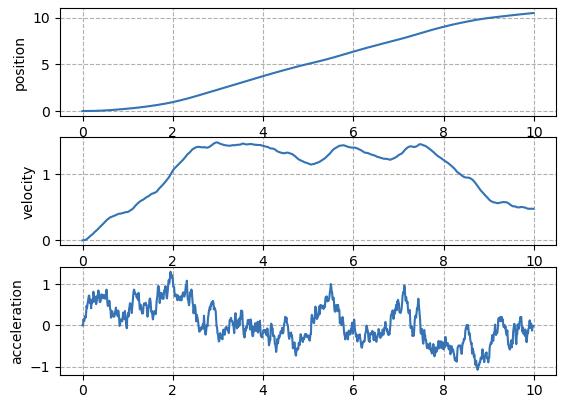
\includegraphics[width=0.56\textwidth]{images/ch1/01OU.jpeg}
    \caption{Change in displacement caused by a randomly generated OU process.}
    \label{fig:01OU}
\end{figure}   





\subsection{Stabilization of Training}
- initiate at close to 0s
- normalization of the data
\subsubsection{Experience Replay}
\subsubsection{Target Network}
\subsubsection{Adaptive Batch Gradient Descent}
\subsubsection{Reward Clipping}
\subsection{Input and State Constraints}
\subsection{Training Algorithm}

%%%%%%%%%%%%%%%%%%%%%%%%%%%%%%%%%% End Section DDPG %%%%%%%%%%%%%%%%%%%%%%%%%%%%%%%%%%%%%%%%
